\documentclass[aps,prd,twocolumn,superscriptaddress,nofootinbib,longbibliography,floatfix,amsmath,amssymb,10pt]{revtex4-2}
\usepackage[utf8]{inputenc}
\usepackage[T1]{fontenc}
\usepackage{mathptmx}
\usepackage{amsthm}
\usepackage{graphicx}
\usepackage{booktabs}
\usepackage{xcolor}
\usepackage[colorlinks=true,linkcolor=blue!50!black,citecolor=blue!50!black,urlcolor=blue!50!black]{hyperref}
\usepackage{orcidlink}
\usepackage[protrusion=true,expansion=false]{microtype}
\usepackage{xurl}
\makeatletter\let\write@bibliographystyle\relax\let\bibliography@latex\@gobble\makeatother
\makeatletter\def\tocdim@min{2.2em}\makeatother
\setcounter{tocdepth}{1}

\theoremstyle{plain}
\newtheorem{theorem}{Theorem}[section]
\newtheorem{proposition}[theorem]{Proposition}
\newtheorem{lemma}[theorem]{Lemma}
\newtheorem{corollary}[theorem]{Corollary}
\theoremstyle{definition}
\newtheorem{definition}[theorem]{Definition}
\newtheorem{remark}[theorem]{Remark}
\theoremstyle{plain}
\newtheorem{mainthm}{Theorem}
\renewcommand{\themainthm}{\Alph{mainthm}}

\newcommand{\EE}{\mathbb{E}}
\newcommand{\cF}{\mathcal{F}}
\newcommand{\qs}{q^{*}}
\newcommand{\Cs}{C^{*}}
\newcommand{\codeDOI}{\href{https://github.com/creelie/eUUR}{\nolinkurl{github.com/creelie/eUUR}}}
\tolerance=2000
\emergencystretch=2em
\hbadness=2000
\hfuzz=1pt
\AtBeginDocument{\setlength{\abovedisplayskip}{6pt plus 1pt minus 2pt}\setlength{\belowdisplayskip}{6pt plus 1pt minus 2pt}\setlength{\abovedisplayshortskip}{3pt plus 1pt}\setlength{\belowdisplayshortskip}{4pt plus 1pt minus 1pt}}

\begin{document}

\title{Attaining the Entropy Limit for Union-Closed Families}

\author{Deep Bhattacharjee\,\orcidlink{0000-0003-0466-750X}}
\email{itsdeep@live.com}
\thanks{Corresponding author. Second address: \nolinkurl{d.bhattacharjee@erl-forschung.de}.}
\affiliation{Formerly, Electro-Gravitational Space Propulsion Laboratory (EGSPL), Bhubaneswar, Odisha 751030, India}
\affiliation{Formerly, University of Calcutta, Senate House, 87/1 College Street, Kolkata 700073, West Bengal, India}

\author{Ushashi Bhattacharya\,\orcidlink{0009-0002-2254-3914}}
\email{rai.bhattacharya.in@gmail.com}
\affiliation{Formerly, National Taiwan University, Taipei 106319, Taiwan}

\date{October 19, 2026}

\begin{abstract}
\itshape
We prove that every finite union-closed family with a nonempty member has an element that lies in at least $0.38288525996\ldots$ of its members. This number is the exact limit of the entropy method in the form developed by Liu and Jiang, and earlier work had come within a hundred-millionth of it without reaching it. The proof chooses the auxiliary function so that the two inequalities behind the method touch zero at a single point, and shows by a convexity argument that they stay nonnegative around it. With a global coupling of Jiang, the bound is strict for every family.
\par\medskip\upshape\noindent\textit{2020 Mathematics Subject Classification.} 05D05; 94A17; 65G30.
\end{abstract}

\keywords{union-closed sets conjecture; Frankl's conjecture; entropy method; interval arithmetic}

\maketitle
\makeatletter\renewcommand\l@subsection[2]{}\renewcommand\l@subsubsection[2]{}\makeatother
\tableofcontents

%----------------------------------------------------------------------
\section{Introduction}\label{sec:intro}

A family $\cF$ of finite sets is \emph{union-closed} if $A\cup B\in\cF$ whenever $A,B\in\cF$. Write $N=|\cF|$ and, for an element $i$ of the ground set,
\[
p_i=\frac{|\{A\in\cF:\ i\in A\}|}{N},\qquad p=\max_i p_i .
\]
Frankl's conjecture states that $p\ge \tfrac12$ whenever $\cF$ contains a nonempty set.\footnote{The conjecture is usually dated to 1979 and attributed to P.~Frankl; the survey of Bruhn and Schaudt \cite{BS15} describes its history, its equivalent lattice and graph forms, and the many special classes for which it is known. The family $\{\emptyset,\{1\}\}$ shows that the constant $\tfrac12$ cannot be raised, and the condition that some member is nonempty only excludes the family $\{\emptyset\}$. Every finite family on an arbitrary ground set can be reduced to one on a finite ground set with the same frequencies for the elements that matter, by keeping one element of a nonempty member and one element of each symmetric difference of two members.} Let $c_{\mathrm{UC}}$ be the largest constant such that $p\ge c_{\mathrm{UC}}$ for every such family.

Until 2022 no positive constant was known. Gilmer \cite{Gil22} then proved $c_{\mathrm{UC}}\ge 0.01$ with a striking entropy argument: two independent uniform members of $\cF$ have a union that is again a member, so its entropy is at most $\ln N$, while a short computation shows that the union has more entropy than either member when all frequencies are small. Within weeks Alweiss, Huang and Sellke \cite{AHS24}, Chase and Lovett \cite{CL22}, Sawin \cite{Saw22} and Pebody \cite{Peb22} pushed the argument to $(3-\sqrt5)/2=0.38196\ldots$. Sawin proposed to couple the two members instead of drawing them independently; Yu \cite{Yu23} and Cambie \cite{Cam22} developed this, and Liu \cite{Liu23} introduced conditionally independent couplings, proved $0.3823455\ldots$ and found numerically that the method should reach $0.382709\ldots$.\footnote{Liu's value $0.382709087918735$ rested on numerically verified hypotheses. Costa \cite{Cos26} and Costa and Sadhu \cite{CS26} proved it, and then, by varying the protocol of Liu's Example~5 and optimising two coefficients, proved $c_{\mathrm{UC}}\ge 0.3828852549667978$. Moffat \cite{Mof26} built a conditionally independent protocol whose kernel has the optimal diagonal and certified $0.38284$ under two numerically checked hypotheses.}

In September 2026 Jiang \cite{Jia26} gave a computer-assisted proof of $c_{\mathrm{UC}}\ge 0.38288525$. Jiang reduced the frequency bound to two scalar inequalities (K) and (M) on the unit square, and showed that no choice of the functions in them can give a constant above
\begin{equation}\label{eq:Cstar}
\Cs=\frac12-\frac{(1-\qs)\ln(1+\qs)}{2\ln 2}=0.3828852599667977965\ldots,
\end{equation}
where $\qs=0.6909077387254077545\ldots$ is the unique root in $(0,1)$ of
\begin{equation}\label{eq:qstar}
(1-q)\ln(1-q)+q\ln(1+q)=0 .
\end{equation}
Costa and Sadhu \cite{CS26} found the same limit for their inequality, and Moffat \cite{Mof26} proved that $\Cs$ bounds every single-letter certificate of this kind whose other protocols admit what Moffat calls component hiding.\footnote{Moffat's refined ceiling $c^{**}=0.382885260\ldots$ coincides with $\Cs$. The argument uses two adversarial laws of the conditional probabilities: a law that puts a tiny atom carrying all the entropy away from the atom where the element is surely absent forces the weight of the independent protocol to be at least $1/(2(1-c))$, and a diagonal two-point law then caps $c$. This ceiling is Moffat's result and we use it only to place ours.} Jiang notes that this theorem does not assert that $\Cs$ itself is achieved; the constant proved there lies $1.0\times10^{-8}$ below it, and that of Costa and Sadhu $5.0\times 10^{-9}$ below it.

We show that the limit is attained.

\begin{mainthm}\label{thm:main}
Every finite union-closed family that contains a nonempty set has an element lying in at least a fraction $\Cs=0.3828852599667977965\ldots$ of its members. In other words, $c_{\mathrm{UC}}\ge\Cs$.
\end{mainthm}

Combining Theorem~\ref{thm:main} with the global coupling of Jiang \cite[Theorem~10.2]{Jia26} gives a strict inequality with an explicit margin for each family.

\begin{mainthm}\label{thm:strict}
If $\cF$ is a union-closed family of size $N\ge 2$ that contains a nonempty set, then
\[
p\ \ge\ \Cs+\frac{\ln^2(2N-1)}{128\,N^2\ln^2 N}\ >\ \Cs .
\]
\end{mainthm}

The margin in Theorem~\ref{thm:strict} tends to zero, so it does not raise $c_{\mathrm{UC}}$ above $\Cs$; by the results just quoted, going further needs an argument outside the single-letter framework. Figure~\ref{fig:records} places the certified constants.

\begin{figure}[t]
\centering
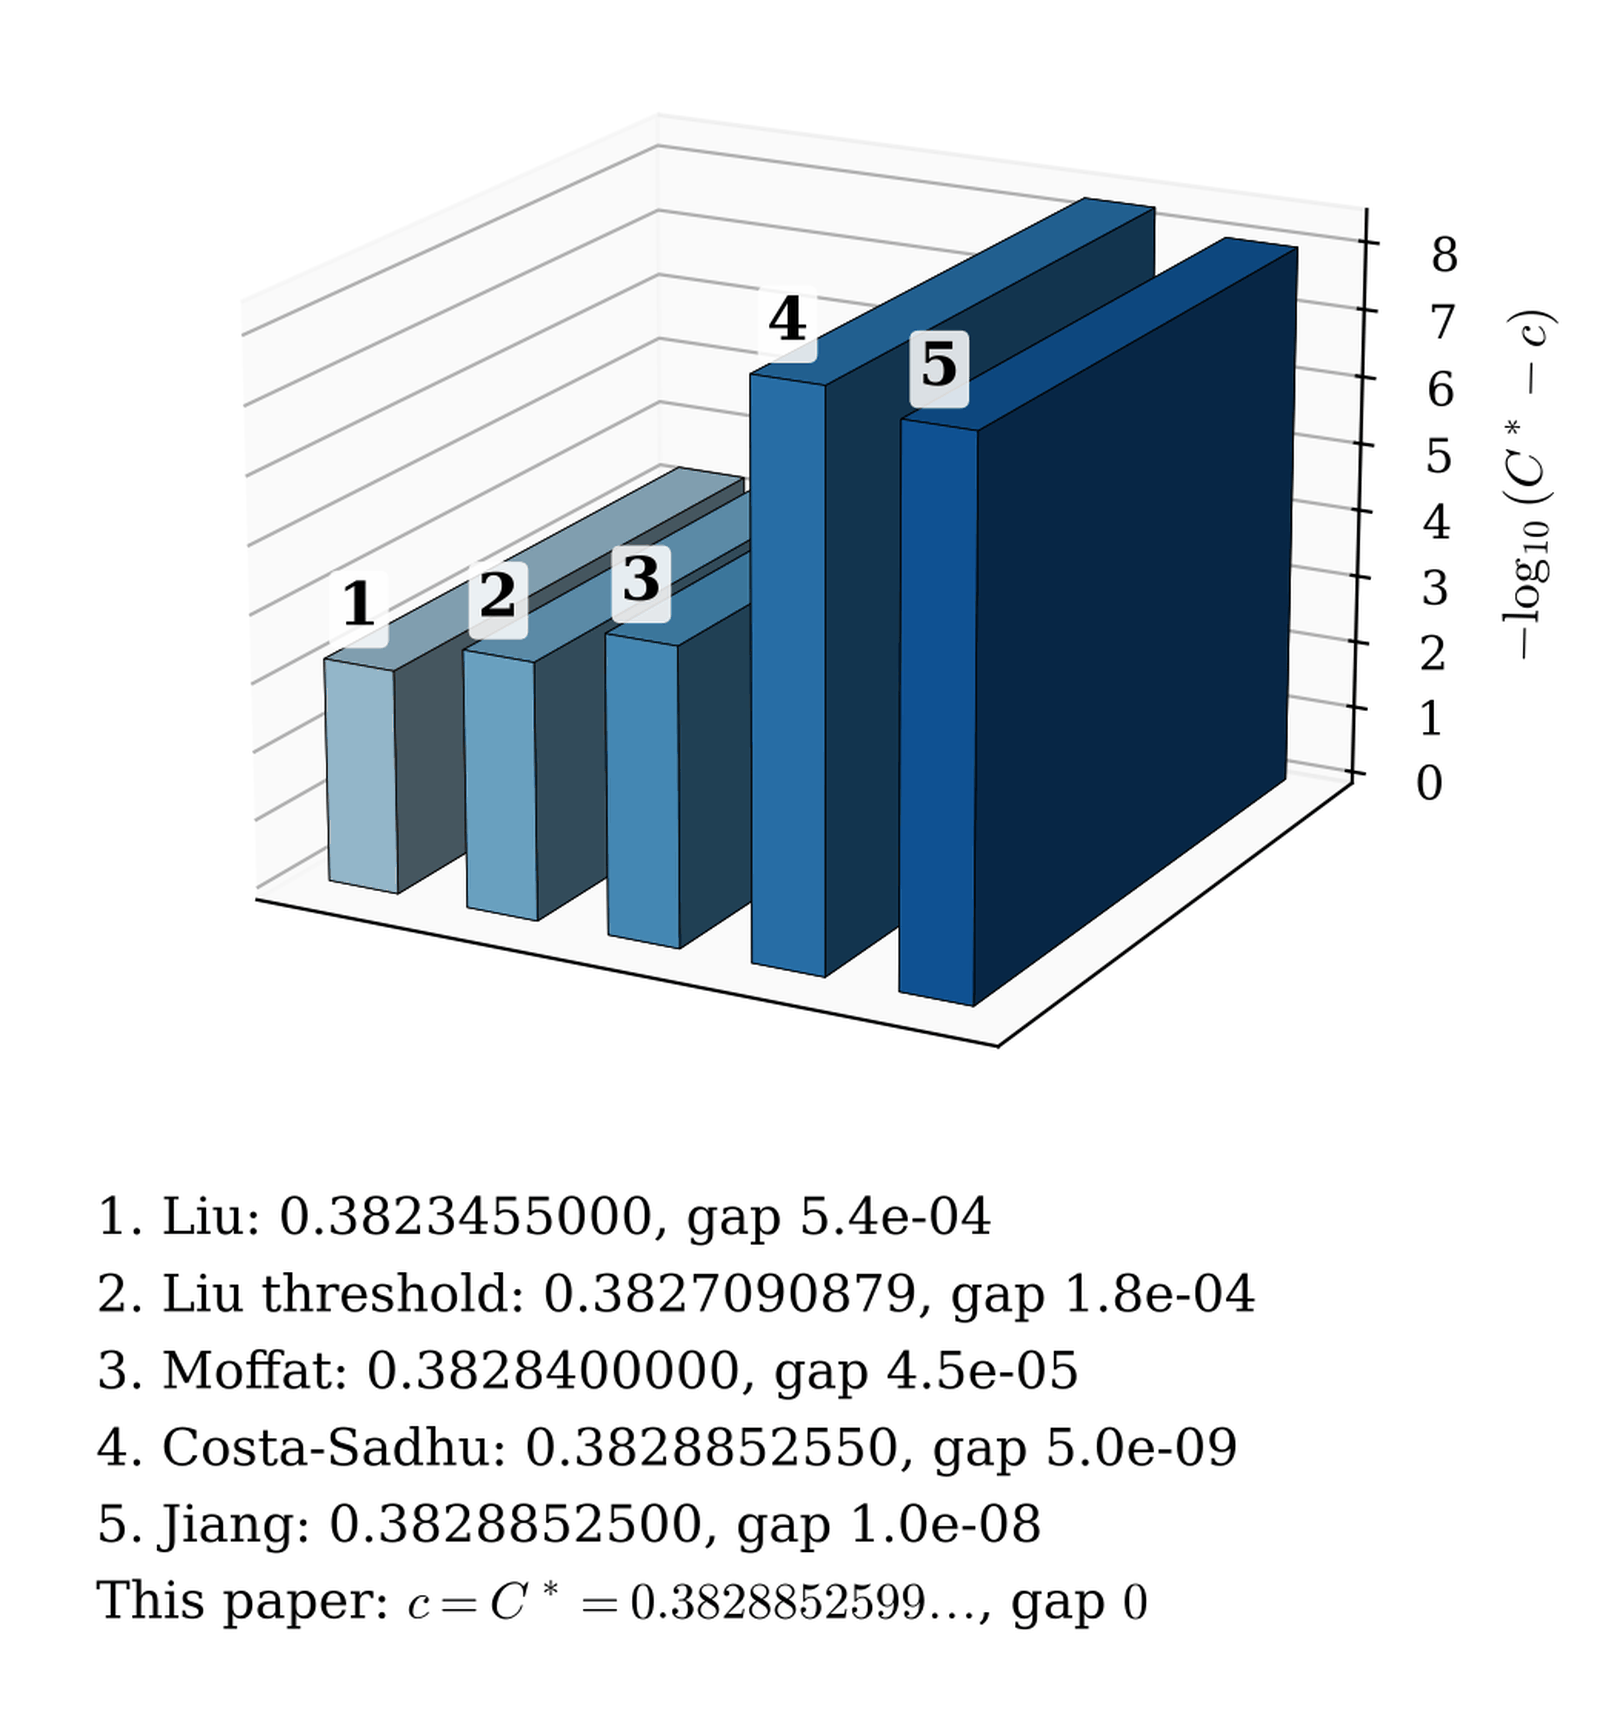
\includegraphics[width=\columnwidth]{figures/fig_records.png}
\caption{Certified lower bounds for $c_{\mathrm{UC}}$ in the entropy line of work, plotted as $-\log_{10}(\Cs-c)$, so that a taller bar is closer to the limit $\Cs$. The bound of this paper is $\Cs$ itself.}
\label{fig:records}
\end{figure}

\paragraph*{Why the limit was not reached before.} At the limit there is no slack anywhere. The constant $\Cs$ comes from two necessary conditions: the edge $y=1$ of (M) forces $mw_0\ge\frac12$, and the diagonal point $x=y=\qs$ of (M) together with $\psi(\qs)^2\le K(\qs,\qs)\le\ln 2$ forces $1-m\le\Cs$. To reach $\Cs$ all three inequalities must be equalities. Then (K) and (M) both vanish at the interior point $(\qs,\qs)$, and an argument that certifies positivity box by box with a fixed margin cannot cover a neighbourhood of that point.\footnote{Jiang kept a margin of order $10^{-8}$ by scaling the profile with $\sigma=0.99999999$ and taking $mw_0=0.500000008685975$; Costa and Sadhu kept a similar margin through a slightly smaller constant. With any positive margin the interval method closes, and the margin can be made as small as the computing budget allows, but it never vanishes.}

\paragraph*{What is new.} We set every parameter to its limiting value: the profile is centred at $\qs$ exactly, its scale is one, and $mw_0=\frac12$ exactly. We then prove that the two gaps vanish to second order at $(\qs,\qs)$, with value and gradient zero (Proposition~\ref{prop:tangent}), and that their Hessians are positive definite on the whole square $[\qs-0.008,\qs+0.008]^2$ (Proposition~\ref{prop:convex}). A function with these two properties is nonnegative on the square. Outside it the inequalities are strict and the interval method of Jiang, rerun with the new parameters, covers the rest; three edge estimates that relied on the old margin turn out to hold with equality allowed (Section~\ref{sec:rest}). Figure~\ref{fig:gaps} shows the two gaps over the unit square.

\begin{figure*}[t]
\centering
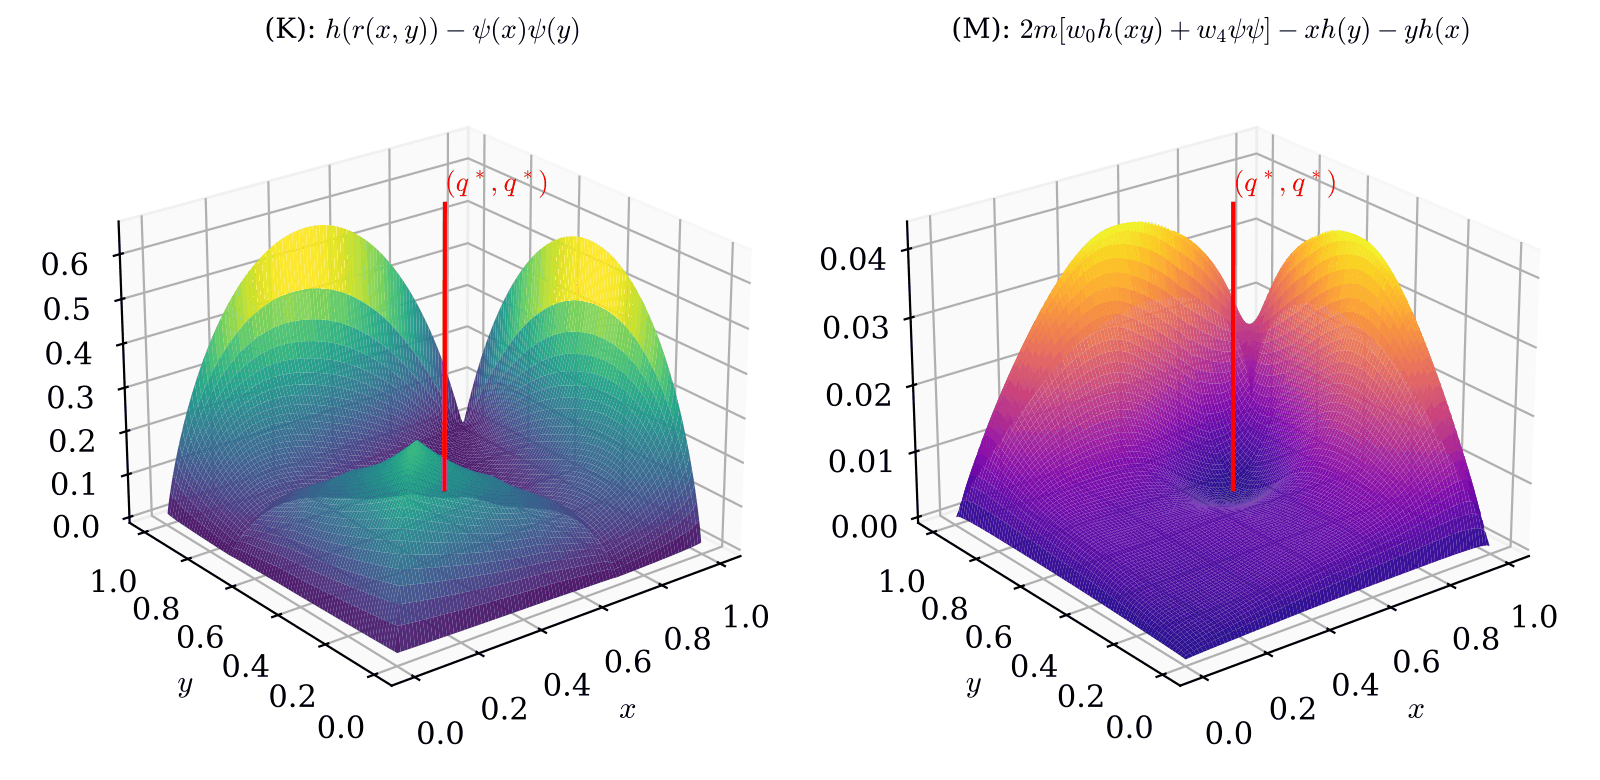
\includegraphics[width=0.92\textwidth]{figures/fig_gaps.png}
\caption{The two gaps of the construction at the limit, over the unit square: on the left the gap $h(r(x,y))-\psi(x)\psi(y)$ of the kernel inequality (K), on the right the gap $2m[w_0h(xy)+w_4\psi(x)\psi(y)]-xh(y)-yh(x)$ of the mixture inequality (M), with $1-m=\Cs$ and $mw_0=\frac12$. Both are nonnegative. Both vanish at the point $(\qs,\qs)$ marked in red; (M) also vanishes on the boundary of the square, where both of its sides are zero, and (K) vanishes on the diagonal above $x=0.721$, where $h(x^2)=s(x)^2$.}
\label{fig:gaps}
\end{figure*}

\paragraph*{Plan.} Section~\ref{sec:reduction} states the entropy reduction. Section~\ref{sec:construction} fixes the functions at the limit and Section~\ref{sec:tangency} proves the contact at $(\qs,\qs)$ and the convexity around it. Section~\ref{sec:rest} covers the rest of the square, Section~\ref{sec:proofs} proves the two theorems and Section~\ref{sec:beyond} discusses what lies beyond $\Cs$. Appendices~\ref{app:reduction} to~\ref{app:strict} give every derivation in full.\footnote{The authors' other work, on analytic estimates in number theory and on modular forms, is in \cite{BNFS26,BB26,BBS23}; the archive of this paper is \cite{BB26z}.}

%----------------------------------------------------------------------
\section{The entropy reduction}\label{sec:reduction}

All logarithms are natural and $h(x)=-x\ln x-(1-x)\ln(1-x)$ is the binary entropy in nats, with $h(0)=h(1)=0$. Let $a:[0,1]\to[0,1]$ and put
\begin{equation}\label{eq:r}
r(x,y)=xy+a(x)a(y)\bigl(\min(x,y)-xy\bigr)
\end{equation}
and $K(x,y)=h\bigl(r(x,y)\bigr)$.
Let $\psi:[0,1]\to[0,\infty)$ and let $w_0,w_4\ge 0$ with $w_0+w_4=1$.\footnote{The index $4$ follows Jiang, who refers to Liu's Example~4; $w_4$ is a weight and not a power. The function $a$ governs how strongly the two samples share randomness: $a\equiv 0$ gives independent bits and $a\equiv 1$ gives bits that are as positively correlated as their marginals allow.}

\begin{proposition}[Jiang \cite{Jia26}, Proposition~3.1]\label{prop:reduction}
Suppose that $m>0$ and that for all $x,y\in[0,1]$
\begin{align}
K(x,y)&\ \ge\ \psi(x)\psi(y), \tag{K}\label{eq:K}\\
2m\bigl[w_0h(xy)+w_4\psi(x)\psi(y)\bigr]&\ \ge\ xh(y)+yh(x). \tag{M}\label{eq:M}
\end{align}
Then every finite union-closed family containing a nonempty set has $p\ge 1-m$.
\end{proposition}

The proof, which we give in full in Appendix~\ref{app:reduction}, runs two sampling rules side by side. The first takes two independent uniform members. The second draws at each coordinate one shared uniform variable and lets each sample's next bit be zero with probability $x+a(x)(\mathbf 1\{U\le x\}-x)$, where $x$ is that sample's conditional probability of a zero; this keeps both samples uniform on $\cF$ and makes the union bit zero with probability $r$. Inequality (K) bounds the entropy of the second union below by a product, conditional independence turns its expectation into a square, and (M) combines the two rules into the bound $w_0H(Z_0)+w_4H(Z_4)\ge \frac{1-p}{m}\ln N$. Both unions lie in $\cF$, so the left side is at most $\ln N$.

The inequalities (K) and (M) cannot hold with $1-m>\Cs$ \cite[Proposition~4.1]{Jia26}; Appendix~\ref{app:limit} repeats the short argument, because its equality cases are exactly the conditions that fix our construction.

%----------------------------------------------------------------------
\section{The construction at the limit}\label{sec:construction}

The construction has the shape of Jiang's, with every parameter at its limiting value. Put
\[
f(q)=q\,h(q)-\tfrac12 h(q^2),
\]
so that $f'(q)=-\bigl[(1-q)\ln(1-q)+q\ln(1+q)\bigr]$ and $\qs$ is the unique maximiser of $f$ on $(0,1)$.\footnote{For $0<q\le\frac12$ one has $f'(q)>q(1-2q)\ge 0$, since $-\ln(1-q)>q>\ln(1+q)$. On $[\frac12,1)$ the function $f'$ is strictly decreasing, because $f''(q)=\ln\frac{1-q}{1+q}+\frac1{1+q}$ is negative at $\frac12$ and $f'''(q)=-\frac{2}{1-q^2}-\frac{1}{(1+q)^2}<0$; it starts at $\frac12\ln\frac43>0$ and tends to $-\ln 2$. So $f'$ has exactly one zero, which is $\qs$. At that zero $(1-\qs)\ln(1-\qs)=-\qs\ln(1+\qs)$, and expanding $h(q^2)$ gives $f(\qs)=\frac12(1-\qs)\ln(1+\qs)$; this is how \eqref{eq:Cstar} arises from $\Cs=\frac12-f(\qs)/\ln2$.} Set
\begin{equation}\label{eq:weights}
mw_0=\tfrac12,\qquad mw_4=\frac{f(\qs)}{\ln 2},\qquad m=\tfrac12+\frac{f(\qs)}{\ln 2}=1-\Cs .
\end{equation}
Thus $w_0=1/(2m)=0.8102221287\ldots$ and $w_4=1-w_0$. The rational breakpoints are
\[
A=\tfrac{179}{250},\quad B=\tfrac{721}{1000},\quad z=\tfrac{181}{256},\quad L=\tfrac1{16},\quad U=\tfrac{15}{16},
\]
with $\frac12<z<\frac1{\sqrt2}<A<B$.\footnote{In integers: $2\cdot181^2=65522<65536=256^2$, $2\cdot179^2=64082>62500=250^2$ and $2\cdot 15^2=450>256$. These order relations, with $z^2+z>1$ and the position of the square $[0.682,0.699]^2$ inside $[\frac12,z]^2$ and below $A$, are checked by the Lean kernel in the archive.} Let
\[
E(x)=-\frac{h'(\qs)}{2h(\qs)}(x-\qs)-\frac{7}{10}(x-\qs)^2
\]
and
\[
D(x)=\begin{cases} h(x), & 0\le x\le \frac12,\\[2pt] \ln 2, & \frac12\le x\le z,\\[2pt] \frac{\ln 2}{h(z^2)}\,h(x^2), & z\le x\le 1,\end{cases}
\]
and define the profile and the upper tail
\begin{equation}\label{eq:phi}
\varphi(x)=\sqrt{\frac{D(x)h(x)}{h(\qs)}}\,e^{E(x)},\quad s(x)=\sqrt{h(x^2)} .
\end{equation}
With $\theta(x)=(x-A)/(B-A)$, the auxiliary function is $\psi=\varphi$ on $[0,A]$, $\psi=(1-\theta)\varphi+\theta s$ on $[A,B]$ and $\psi=s$ on $[B,1]$. The sampling coefficient is
\begin{equation}\label{eq:a}
a(x)=\begin{cases}1, & 0\le x\le\frac12,\\[2pt] \sqrt{\dfrac{1-2x^2}{2x(1-x)}}, & \frac12<x<\frac1{\sqrt2},\\[6pt] 0, & \frac1{\sqrt2}\le x\le 1.\end{cases}
\end{equation}

Jiang takes the centre $x^*=0.690908$, the scale $\sigma=0.99999999$ and $mw_0>\frac12$; here the centre is $\qs$, the scale is $1$ and the weights are \eqref{eq:weights}.\footnote{The centre $\qs$ is an irrational number given by \eqref{eq:qstar}. It is never approximated by a rational number in the proof: the interval computation carries an enclosure of $\qs$ of radius $10^{-30}$ about $0.690907738725407754557261116505$, obtained from a certified sign change of $f'$, and every quantity that depends on $\qs$ is evaluated over this interval. Since $f'$ is strictly decreasing near $\qs$, the sign change proves that $\qs$ lies in the interval.} The middle formula of \eqref{eq:a} is chosen so that
\begin{equation}\label{eq:rdiag}
r(q,q)=q^2+a(q)^2\,q(1-q)=\tfrac12\qquad\Bigl(\tfrac12\le q\le\tfrac{1}{\sqrt2}\Bigr),
\end{equation}
so the shared-randomness union bit has the largest possible entropy $\ln 2$ on that part of the diagonal.

%----------------------------------------------------------------------
\section{Contact at one point and convexity around it}\label{sec:tangency}

Write
\begin{align*}
G_K(x,y)&=K(x,y)-\psi(x)\psi(y),\\
G_M(x,y)&=h(xy)+2mw_4\psi(x)\psi(y)-xh(y)-yh(x),
\end{align*}
so that (K) and (M) say $G_K\ge 0$ and $G_M\ge 0$ (for (M) we used $2mw_0=1$). Let $S=[\qs-0.008,\qs+0.008]^2$. On $S$ every coordinate lies in $[0.682,0.699]\subset(\frac12,z)$ and below $A$, so $\psi=\varphi$, $D=\ln 2$ and $a$ is given by its middle formula. On each of the two closed triangles of $S$ cut by the diagonal, $G_K$ agrees with one of the smooth functions
\begin{align*}
G_K^{(1)}(x,y)&=h\bigl(xy+a(x)a(y)(x-xy)\bigr)-\varphi(x)\varphi(y),\\
G_K^{(2)}(x,y)&=G_K^{(1)}(y,x),
\end{align*}
the first on $x\le y$ and the second on $x\ge y$.

\begin{proposition}\label{prop:tangent}
The functions $G_K^{(1)}$, $G_K^{(2)}$ and $G_M$ vanish at $(\qs,\qs)$, and so do their gradients.
\end{proposition}

\begin{proof}
By \eqref{eq:rdiag}, $r(\qs,\qs)=\frac12$, so $K(\qs,\qs)=\ln 2$. Since $D(\qs)=\ln 2$ and $E(\qs)=0$, \eqref{eq:phi} gives $\varphi(\qs)^2=\ln 2$; hence $G_K^{(i)}(\qs,\qs)=0$. The logarithmic derivative of $\varphi$ on $(\frac12,z)$ is $\frac{h'}{2h}+E'$, and $E'(\qs)=-\frac{h'(\qs)}{2h(\qs)}$; so $\varphi'(\qs)=0$. The gradient of $h(r)$ is $h'(r)\nabla r$, which vanishes at $(\qs,\qs)$ because $h'(\frac12)=0$. The gradient of $\varphi(x)\varphi(y)$ is $(\varphi'(x)\varphi(y),\varphi(x)\varphi'(y))$, also zero there.

For $G_M$, the value at $(\qs,\qs)$ is
\[
h({\qs}^2)+2mw_4\ln2-2\qs h(\qs)=2mw_4\ln 2-2f(\qs)=0
\]
by \eqref{eq:weights}. Its partial derivative in $x$ is
\[
y\,h'(xy)+2mw_4\varphi'(x)\varphi(y)-h(y)-y\,h'(x),
\]
which at $(\qs,\qs)$ equals $\qs h'({\qs}^2)-h(\qs)-\qs h'(\qs)=-f'(\qs)=0$; by symmetry the partial derivative in $y$ is also zero.
\end{proof}

At $(\qs,\qs)$ the Hessians have closed forms (Appendix~\ref{app:hessian}). Put $\alpha=a(\qs)^2=\frac{1-2{\qs}^2}{2\qs(1-\qs)}$ and let $\kappa=(\ln\varphi)''(\qs)$. Then
\begin{align}
\nabla^2G_K^{(i)}(\qs,\qs)&=-\alpha^2\begin{pmatrix}1&-1\\-1&1\end{pmatrix}-\kappa\ln 2\,I,\label{eq:HK}\\
\nabla^2G_M(\qs,\qs)&=\begin{pmatrix}\beta&\gamma\\ \gamma&\beta\end{pmatrix},\label{eq:HM}
\end{align}
where $I$ is the identity matrix, $\beta={\qs}^2h''({\qs}^2)+2f(\qs)\kappa-\qs h''(\qs)$ and $\gamma=h'({\qs}^2)+{\qs}^2h''({\qs}^2)-2h'(\qs)$. Numerically $\alpha=0.10604564\ldots$, $\kappa=-6.03228523\ldots$, the matrix \eqref{eq:HK} has diagonal $4.17001582\ldots$ and off-diagonal $0.01124567\ldots$, and \eqref{eq:HM} has $\beta=0.34256611\ldots$ and $\gamma=-0.21395816\ldots$. All three are positive definite. Figure~\ref{fig:tangency} shows the two gaps near the point of contact.

\begin{figure*}[t]
\centering
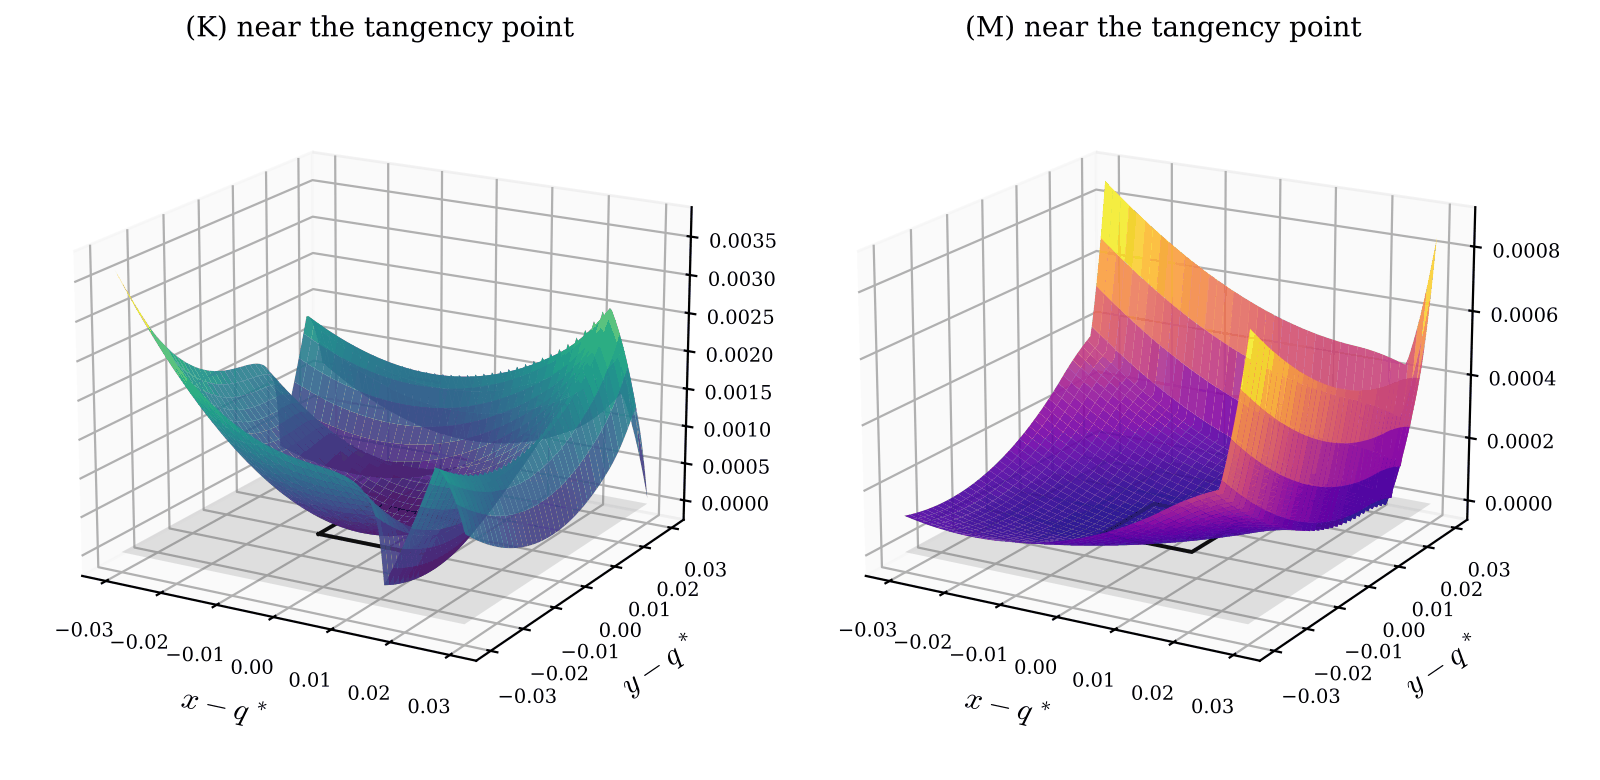
\includegraphics[width=0.92\textwidth]{figures/fig_tangency.png}
\caption{The gaps of (K) and (M) on $[\qs-0.03,\qs+0.03]^2$, plotted against $(x-\qs,y-\qs)$. Each surface touches the grey plane of height zero only at the origin. The black square is the boundary of $S=[\qs-0.008,\qs+0.008]^2$, on which the Hessians are certified positive definite. The ridge of the left surface along the diagonal is the kink of $\min(x,y)$ in \eqref{eq:r}.}
\label{fig:tangency}
\end{figure*}

\begin{proposition}\label{prop:convex}
The Hessians of $G_K^{(1)}$, $G_K^{(2)}$ and $G_M$ are positive definite at every point of $S$. Consequently $G_K\ge 0$ and $G_M\ge 0$ on $S$.
\end{proposition}

\begin{proof}
Divide $S$ into $40\times 40$ congruent closed squares. On each of them we enclose the three second derivatives of each function by second-order forward differentiation in ball arithmetic with $200$-bit precision, and check that the enclosures satisfy $f_{xx}>0$, $f_{yy}>0$ and $f_{xx}f_{yy}-f_{xy}^2>0$ for every choice of the entries in their balls. This implies positive definiteness at every point of the small square. Table~\ref{tab:hessian} lists the extreme values over all $1600$ squares.

A twice differentiable function $g$ on a convex set with positive definite Hessian is convex. If moreover $g(p_0)=0$ and $\nabla g(p_0)=0$ at an interior point $p_0$, then $g(p)\ge g(p_0)+\nabla g(p_0)\cdot(p-p_0)=0$ for every $p$ in the set. Apply this to $G_K^{(1)}$, $G_K^{(2)}$ and $G_M$ on $S$ with $p_0=(\qs,\qs)$, using Proposition~\ref{prop:tangent}. Since $G_K$ equals $G_K^{(1)}$ or $G_K^{(2)}$ at each point of $S$, both gaps are nonnegative on $S$.
\end{proof}

\begin{table}[t]
\centering
\caption{Enclosures of the Hessians over the $1600$ subsquares of $S$. The entries are the smallest lower bounds of $g_{xx}$, $g_{yy}$ and of the determinant, and the largest bound of $|g_{xy}|$.}
\label{tab:hessian}
\begin{tabular}{lcccc}
\toprule
function & $\min g_{xx}$ & $\min g_{yy}$ & $\max|g_{xy}|$ & $\min\det$\\
\midrule
$G_K^{(1)}$ & $2.321$ & $2.092$ & $1.139$ & $5.663$\\
$G_K^{(2)}$ & $2.092$ & $2.321$ & $1.139$ & $5.663$\\
$G_M$ & $0.3114$ & $0.3114$ & $0.2303$ & $0.0587$\\
\bottomrule
\end{tabular}
\end{table}

The radius $0.008$ is close to the largest that works for (K). The second derivatives of $a$ grow without bound as $x\to 1/\sqrt2=0.7071\ldots$, and at radius $0.01$ the enclosures over squares near the upper corner of $S$ are no longer positive definite.\footnote{This is a limitation of the enclosure and not of the inequality: $G_K$ is positive at every point of $[0.682,0.701]^2$ other than $(\qs,\qs)$. The radius only has to be large enough for the box method of Section~\ref{sec:rest} to cover the complement of $S$, where both gaps are strictly positive.}

%----------------------------------------------------------------------
\section{The rest of the unit square}\label{sec:rest}

Away from $S$ both gaps are strictly positive, and the covering of Jiang \cite[Sections~6--9]{Jia26} applies with the new parameters. It splits the work into analytic estimates near the boundary of each domain and a box-by-box interval computation on the compact remainder. Figure~\ref{fig:scheme} shows the layout. We list the parts and the scalar inequalities they rest on; Appendix~\ref{app:analytic} gives every estimate in full with the present parameters.

\begin{figure*}[t]
\centering
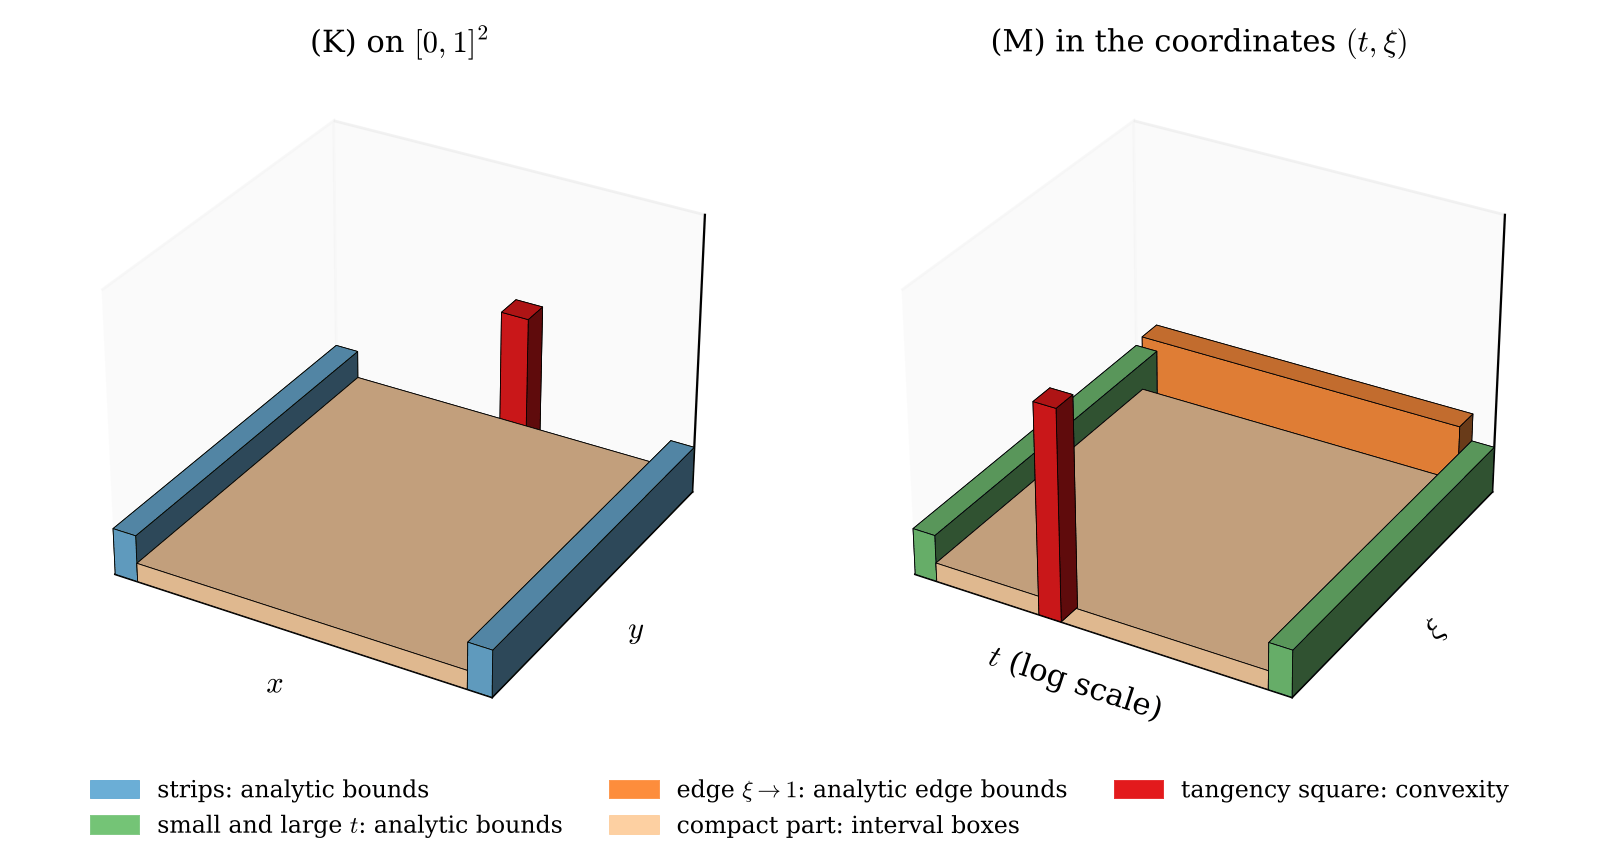
\includegraphics[width=0.92\textwidth]{figures/fig_scheme.png}
\caption{How the two domains are covered. Left: the unit square of (K), with the lower and upper strips $x\le\frac1{16}$ and $x\ge\frac{15}{16}$ handled analytically, the compact square handled by interval boxes in Jiang's three coordinate maps, and the square $S$ around $(\qs,\qs)$ handled by convexity. Right: the domain of (M) in the coordinates $x=e^{-t(1+\xi)}$, $y=e^{-t(1-\xi)}$, with analytic bounds for $t<0.001$, for $t\ge 16$ and near the edge $\xi\to 1$, interval boxes elsewhere, and the image of $S$ handled by convexity.}
\label{fig:scheme}
\end{figure*}

\paragraph*{The kernel inequality.} It suffices to prove $K\ge\varphi(x)\varphi(y)$ on the whole square, together with the bridge $h(Ay)\ge s(A)\varphi(y)$ for $0\le y\le A$ and the inequality $\varphi\le\psi\le s$ on $[A,1]$; the passage to $\psi$ then uses the geometric concavity $h(xy)\ge s(x)s(y)$ (Lemma~\ref{lem:geom}). The strips $x\le L$ and $x\ge U$ are handled by the constants
\begin{gather*}
C_b=\frac{e^{E(L)}}{\sqrt{h(\qs)}},\qquad P_0=\frac{\ln2\,e^{E(1/2)}}{\sqrt{h(\qs)}},\\
C_g=\sqrt{\frac{2\ln 2}{h(\qs)h(z^2)}}\,e^{E(1)},\quad C_t=\frac1U\sqrt{\frac{\ln2\,h(U^2)h(U)}{h(z^2)h(\qs)}}\,e^{E(1)},
\end{gather*}
through the scalar inequalities of Table~\ref{tab:scalars}. The compact square $[L,U]^2$ is covered by boxes in Jiang's parametrisation of the middle interval by $t=a(x)$, which removes the singularity of $a'$ at $1/\sqrt 2$. Boxes contained in $S$ are accepted by Proposition~\ref{prop:convex}.

\paragraph*{The mixture inequality.} With $x=e^{-u}$, $y=e^{-v}$, $u=t(1+\xi)$, $v=t(1-\xi)$, $G(u)=e^{u}h(e^{-u})$ and $P(u)=e^{u}\psi(e^{-u})$, inequality (M) on the half square $x\le y$ is equivalent to
\begin{equation}\label{eq:F}
F(t,\xi)=\tfrac12G(2t)+mw_4P(u)P(v)-\tfrac12\bigl(G(u)+G(v)\bigr)\ \ge\ 0
\end{equation}
for $t>0$, $0\le\xi\le1$. For $t\le 0.001$ the bound $G(u)+G(v)-G(u+v)\le 2\sqrt{uv}$ and $P=\sqrt{G(2\,\cdot)}$ give $F\ge\bigl[2mw_4(1-\ln 0.004)-1\bigr]\sqrt{uv}\ge0$. For $t\ge 16$ the lower bound $\psi\ge C h$ with $C=e^{E(0)}/\sqrt{h(\qs)}$ gives $F\ge(16\,mw_4C^2-\frac12)G(v)\ge0$. Near the edge $\xi\to 1$, where $v\to 0$, two estimates give $F\ge(mw_0-\frac12)G(2t)$, which is $0$ by \eqref{eq:weights}; this suffices, because the acceptance test only needs $F\ge 0$. The remaining rectangle $[0.001,16]\times[0,1]$ is covered by interval boxes, and boxes whose image lies in $S$ are accepted by Proposition~\ref{prop:convex}.

\begin{table}[t]
\centering
\caption{The scalar inequalities used by the analytic parts, each checked by interval arithmetic with the parameters of Section~\ref{sec:construction}. Every margin is the lower end of a certified enclosure.}
\label{tab:scalars}
\begin{tabular}{lr}
\toprule
inequality & certified margin\\
\midrule
$E'(1)>0$ & $0.21766$\\
$1-C_gC_t>0$ & $0.06286$\\
$1-C_bP_0>0$ & $0.51357$\\
$1-2C_bP_0>0$ & $0.02714$\\
$1-E'(\frac12)-h'(z^2)/h(z^2)>0$ & $0.08172$\\
$A-s(A)C_b>0$ & $0.18250$\\
$s(A)-\varphi(A)>0$ & $0.00164$\\
$-\bigl(\frac{h'(A)}{2h(A)}+E'(A)\bigr)>0$ & $0.15960$\\
$2mw_4(1-\ln 0.004)-1>0$ & $0.52752$\\
$e^{-0.002}-B>0$ & $0.27700$\\
$16\,mw_4C^2-\frac12>0$ & $0.13232$\\
\bottomrule
\end{tabular}
\end{table}

\paragraph*{The computation.} Every quantity is an interval with outward rounding at $35$ significant digits. A box is accepted when the interval value of the gap has a positive lower end, or when the value at its centre minus the derivative bound times the radius is positive, or when an analytic edge bound or Proposition~\ref{prop:convex} applies; otherwise it is bisected. A completed run accepts every descendant of the initial boxes, which proves coverage. Table~\ref{tab:run} records the run; it takes about ninety seconds on one processor.

\begin{table}[t]
\centering
\caption{The interval verification at the limit. ``Convex'' counts the boxes accepted because they lie in $S$; ``edge'' counts the mixture boxes accepted by the edge estimates. The smallest margin is over the boxes accepted with a positive lower bound.}
\label{tab:run}
\begin{tabular}{lrrrrl}
\toprule
part & boxes & leaves & convex & edge & smallest margin\\
\midrule
bridge & $39$ & $20$ & -- & -- & $4.60\times10^{-6}$\\
kernel & $1572$ & $789$ & $53$ & -- & $1.44\times10^{-7}$\\
mixture & $8193$ & $4101$ & $23$ & $91$ & $7.10\times10^{-8}$\\
\bottomrule
\end{tabular}
\end{table}

%----------------------------------------------------------------------
\section{Proof of the theorems}\label{sec:proofs}

\begin{proof}[Proof of Theorem~\ref{thm:main}]
By Proposition~\ref{prop:convex}, (K) and (M) hold on $S$. On the rest of the unit square they hold by Section~\ref{sec:rest} and Appendix~\ref{app:analytic}: (K) by the strips, the compact square, the bridge and the upper tail, and (M) on $x\le y$ by the small and large $t$ estimates, the edge estimates and the compact rectangle, and on $x>y$ by symmetry, while both sides of (M) vanish when $xy=0$ or $x=y=1$. Proposition~\ref{prop:reduction} with $1-m=\Cs$ gives $p\ge\Cs$.
\end{proof}

\begin{proof}[Proof of Theorem~\ref{thm:strict}]
Appendix~\ref{app:strict} repeats Jiang's argument \cite[Proposition~10.3]{Jia26} with the present parameters. It gives $p\ge 1-m+mw_0V/(16\ln^2N)$, where $V\ge\ln^2(2N-1)/(4N^2)$ is a variance of logarithms of union multiplicities. With $1-m=\Cs$ and $mw_0=\frac12$ this is the stated bound.
\end{proof}

%----------------------------------------------------------------------
\section{Beyond the limit}\label{sec:beyond}

Theorem~\ref{thm:main} closes the gap between what the reduction (K)--(M) can certify and what has been certified with it. Further progress on Frankl's conjecture through entropy needs a different inequality. Three facts constrain the search.\footnote{We record them because they decide where effort is useful. None of them is new: the first is Jiang's Proposition~4.1 \cite{Jia26}, the second and third are the two ceilings of Moffat \cite{Mof26}.} First, the edge $y=1$ of (M) and the diagonal bound $\psi^2\le\ln2$ alone force $1-m\le\Cs$, whatever $a$ and $\psi$ are, and the same holds for any finite sum of products $\psi_j(x)\psi_j(y)$. Second, any single-letter certificate that uses the independent protocol and other protocols admitting component hiding is bounded by $\Cs$. Third, any single-letter certificate whose classes contain product laws is bounded by $1-h(1/\sqrt2)/\sqrt2=0.383099\ldots$.

A useful structural fact holds for every union-closed family: if the next bit of a prefix $\alpha$ is forced to be zero, so is the next bit of every prefix $\alpha'\subseteq\alpha$ that occurs.\footnote{If $\alpha'\subseteq\alpha$ are both prefixes of members and some member extending $\alpha'$ had bit $1$ at the next coordinate, its union with a member extending $\alpha$ would extend $\alpha$ and have bit $1$ there.} So the set of prefixes at which an element is surely absent is a down-set. The adversarial laws behind the ceilings place such prefixes freely. An argument that uses the down-set structure, for instance through a correlation inequality of Harris type across coordinates, is not covered by the ceilings; we do not know whether it gives more.

%----------------------------------------------------------------------
\section*{Data and code availability}
The interval programs, the Hessian certification, independent checks in C, C\texttt{++} and Julia, the Lean~4 check of the rational breakpoints, the figure programs and the \LaTeX{} source are in the repository \codeDOI{} and its Zenodo archive \cite{BB26z}. Deep Bhattacharjee carried out the computations and the Python, C, C\texttt{++}, Julia, Lean and shell verifications with AI assistance (Claude, Anthropic).

\section*{Ethical declarations}
Funding: none. Competing interests: none.

\section*{Author contributions}
Deep Bhattacharjee proposed the problem, carried out the computations and wrote the paper. Ushashi Bhattacharya checked the derivations of the appendices. Both authors approved the final version.

\appendix

%----------------------------------------------------------------------
\section{Proof of the entropy reduction}\label{app:reduction}

This appendix proves Proposition~\ref{prop:reduction}, following Gilmer \cite{Gil22}, Liu \cite{Liu23} and Jiang \cite{Jia26}. We use two elementary facts about $h$: it is concave, so $h(\lambda x)\ge\lambda h(x)$ for $\lambda\in[0,1]$, and conditioning reduces entropy.

\paragraph*{Native conditional probabilities.} Let $\cF\subseteq 2^{[n]}$ with $N\ge 2$ and let $X$ be uniform on $\cF$, viewed as a $0$--$1$ vector. For a prefix $\alpha\in\{0,1\}^{i-1}$ set $x_i(\alpha)=\Pr(X_i=0\mid X_{<i}=\alpha)$, and let $P_i$ be the law of $x_i(X_{<i})$. Then
\begin{equation}\label{eq:native}
\EE_{P_i}x=1-p_i,\qquad \EE_{P_i}h(x)=H(X_i\mid X_{<i}),
\end{equation}
where $p_i$ is the frequency of element $i$.

\paragraph*{The independent rule.} Take two independent copies $X^{(0)}$ and $Y^{(0)}$ of $X$, and let $Z_0=X^{(0)}\vee Y^{(0)}$, the coordinatewise maximum, which is the indicator of the union. Given both prefixes at coordinate $i$, the two bits are independent with zero probabilities $S=x_i(X^{(0)}_{<i})$ and $T=x_i(Y^{(0)}_{<i})$, so the union bit is zero with probability $ST$. The prefix of $Z_0$ is a function of the two prefixes, so
\begin{equation}\label{eq:Z0}
H\bigl((Z_0)_i\mid(Z_0)_{<i}\bigr)\ \ge\ H\bigl((Z_0)_i\mid X^{(0)}_{<i},Y^{(0)}_{<i}\bigr)=\EE_{P_i\otimes P_i}h(ST).
\end{equation}

\paragraph*{The shared rule.} At each coordinate $i$ draw a fresh uniform $U_i$ on $[0,1]$, shared by the two samples, and set $Q_{U}(x)=x+a(x)(\mathbf 1\{U\le x\}-x)$. Given $U_i$ and the two prefixes, generate the two bits independently with zero probabilities $Q_{U_i}(S)$ and $Q_{U_i}(T)$, where $S,T$ are the native probabilities of the two prefixes. Since $\EE_U Q_U(x)=x$ and $U_i$ is independent of each prefix, each sample has its native transition law at every step, so by induction each of $X^{(4)},Y^{(4)}$ is uniform on $\cF$. Since $\EE\,\mathbf 1\{U\le x\}\mathbf 1\{U\le y\}=\min(x,y)$,
\[
\EE_U\bigl[Q_U(x)Q_U(y)\bigr]=xy+a(x)a(y)\bigl(\min(x,y)-xy\bigr)=r(x,y),
\]
so given the prefixes the union bit of $Z_4=X^{(4)}\vee Y^{(4)}$ is zero with probability $r(S,T)$ and has entropy $K(S,T)$.

\paragraph*{Conditional independence.} The shared variables used before coordinate $i$ form the vector $V_i=(U_1,\dots,U_{i-1})$. Given $V_i$, the two prefixes are functions of $V_i$ and of independent local randomness, so they are independent and identically distributed; hence so are $S$ and $T$. Therefore
\[
\EE[\psi(S)\psi(T)]=\EE\Bigl[\bigl(\EE[\psi(S)\mid V_i]\bigr)^2\Bigr]\ge\bigl(\EE\psi(S)\bigr)^2=\bigl(\EE_{P_i}\psi\bigr)^2,
\]
by the nonnegativity of a variance. With (K) and conditioning,
\begin{equation}\label{eq:Z4}
H\bigl((Z_4)_i\mid(Z_4)_{<i}\bigr)\ \ge\ \EE K(S,T)\ \ge\ \bigl(\EE_{P_i}\psi\bigr)^2 .
\end{equation}

\paragraph*{Combination.} Integrate (M) against $P_i\otimes P_i$. The right side becomes $2(\EE_{P_i}x)(\EE_{P_i}h)=2(1-p_i)H(X_i\mid X_{<i})$ by \eqref{eq:native}, and the product term on the left becomes $(\EE_{P_i}\psi)^2$ because the two variables are independent. Dividing by $2m$,
\[
w_0\,\EE_{P_i\otimes P_i}h(ST)+w_4\bigl(\EE_{P_i}\psi\bigr)^2\ \ge\ \frac{1-p_i}{m}\,H(X_i\mid X_{<i}).
\]
By \eqref{eq:Z0} and \eqref{eq:Z4}, summing over $i$ and using the chain rule,
\[
w_0H(Z_0)+w_4H(Z_4)\ \ge\ \sum_{i=1}^n\frac{1-p_i}{m}H(X_i\mid X_{<i})\ \ge\ \frac{1-p}{m}\ln N,
\]
since $1-p_i\ge 1-p$ and $\sum_iH(X_i\mid X_{<i})=H(X)=\ln N$. Union closure puts $Z_0$ and $Z_4$ in $\cF$, so each has entropy at most $\ln N$ and the left side is at most $\ln N$. Dividing by $\ln N>0$ gives $p\ge 1-m$. If $N=1$ the only member is nonempty and some element has frequency $1$.

%----------------------------------------------------------------------
\section{Why the limit is \texorpdfstring{$\Cs$}{C*}}\label{app:limit}

Suppose (K) and (M) hold. Since $r(1,1)=1$, (K) gives $\psi(1)^2\le h(1)=0$, so $\psi(1)=0$. Put $y=1$ in (M): the left side is $2mw_0h(x)$ and the right side is $h(x)$, so
\begin{equation}\label{eq:edge}
mw_0\ \ge\ \tfrac12 .
\end{equation}
Put $x=y=q$ in (M) and use $\psi(q)^2\le K(q,q)\le\ln 2$ and $w_4=1-w_0$:
\begin{align*}
2q\,h(q)&\le 2mw_0h(q^2)+2(m-mw_0)\ln 2\\
&= 2m\ln2-2mw_0\bigl(\ln2-h(q^2)\bigr)\\
&\le 2m\ln 2-\ln2+h(q^2),
\end{align*}
using \eqref{eq:edge} and $h(q^2)\le\ln 2$. Hence $1-m\le\frac12-f(q)/\ln2$ for every $q$, and the best choice $q=\qs$ gives $1-m\le\Cs$.

Equality $1-m=\Cs$ therefore requires $mw_0=\frac12$, $\psi(\qs)^2=K(\qs,\qs)=\ln 2$, and equality in (M) at $(\qs,\qs)$. These are exactly the conditions imposed in Section~\ref{sec:construction}. Since $G_K$ and $G_M$ are nonnegative and vanish at the interior point $(\qs,\qs)$, their gradients must vanish there too, so Proposition~\ref{prop:tangent} is forced as well; what has to be shown is the second-order condition.

%----------------------------------------------------------------------
\section{The Hessians at the point of contact}\label{app:hessian}

We derive \eqref{eq:HK} and \eqref{eq:HM}. Throughout, $q=\qs$, $h'(u)=\ln\frac{1-u}{u}$ and $h''(u)=-\frac{1}{u(1-u)}$.

\paragraph*{The profile.} On $(\frac12,z)$ we have $\ln\varphi=\frac12\ln\ln 2+\frac12\ln h-\frac12\ln h(q)+E$, so
\[
(\ln\varphi)'=\frac{h'}{2h}+E',\qquad (\ln\varphi)''=\frac{h''h-h'^2}{2h^2}-\frac75 .
\]
At $q$ the first derivative is zero. Since $\varphi''/\varphi=(\ln\varphi)''+((\ln\varphi)')^2$, we get $\varphi''(q)\varphi(q)=\kappa\,\varphi(q)^2=\kappa\ln 2$ with
\[
\kappa=\frac{h''(q)h(q)-h'(q)^2}{2h(q)^2}-\frac75=-6.0322852376\ldots
\]

\paragraph*{The gradient of $r$.} On the branch $\min(x,y)=x$ we have $r=xy+a(x)a(y)(x-xy)$, so at $(q,q)$, writing $a=a(q)$ and $a'=a'(q)$,
\[
r_x=q+aa'q(1-q)+a^2(1-q),\quad r_y=q+aa'q(1-q)-a^2q .
\]
Differentiating the identity $a(x)^2x(1-x)=\frac12-x^2$ at $q$ gives $2aa'q(1-q)+a^2(1-2q)=-2q$, that is $aa'q(1-q)=-q-\frac12\alpha(1-2q)$ with $\alpha=a^2$. Substituting,
\[
r_x=\tfrac12\alpha,\qquad r_y=-\tfrac12\alpha .
\]
On the other branch the roles are exchanged and $\nabla r=(-\frac12\alpha,\frac12\alpha)$.

\paragraph*{The kernel gap.} The Hessian of $h(r)$ is $h''(r)\nabla r\,\nabla r^{\mathsf T}+h'(r)\nabla^2r$. At $(q,q)$, $r=\frac12$, $h'(\frac12)=0$ and $h''(\frac12)=-4$, so the Hessian of $h(r)$ is $-4\nabla r\nabla r^{\mathsf T}=-\alpha^2\bigl(\begin{smallmatrix}1&-1\\-1&1\end{smallmatrix}\bigr)$ on either branch. The Hessian of $\varphi(x)\varphi(y)$ at $(q,q)$ is $\bigl(\begin{smallmatrix}\varphi''\varphi&\varphi'^2\\ \varphi'^2&\varphi\varphi''\end{smallmatrix}\bigr)=\kappa\ln 2\,I$. Subtracting gives \eqref{eq:HK}. Its eigenvalues are $-\kappa\ln 2=4.1812\ldots$ on the vector $(1,1)$ and $-2\alpha^2-\kappa\ln2=4.1588\ldots$ on $(1,-1)$, both positive.

\paragraph*{The mixture gap.} On $S$ the mixture gap is $G_M=h(xy)+2mw_4\varphi(x)\varphi(y)-xh(y)-yh(x)$. Differentiating twice,
\begin{align*}
\partial_{xx}G_M&=y^2h''(xy)+2mw_4\varphi''(x)\varphi(y)-y\,h''(x),\\
\partial_{xy}G_M&=h'(xy)+xy\,h''(xy)+2mw_4\varphi'(x)\varphi'(y)\\&\quad-h'(y)-h'(x).
\end{align*}
At $(q,q)$, with $\varphi'(q)=0$, $\varphi''(q)\varphi(q)=\kappa\ln2$ and $mw_4\ln 2=f(q)$, these become $\beta$ and $\gamma$ of \eqref{eq:HM}. Numerically $\beta=0.3425661126\ldots$ and $\gamma=-0.2139581685\ldots$, so the eigenvalues $\beta+\gamma=0.1286\ldots$ and $\beta-\gamma=0.5565\ldots$ are positive.

\paragraph*{From the point to the square.} Positive definiteness at $(q,q)$ gives nonnegativity only in some neighbourhood of unknown size. Proposition~\ref{prop:convex} makes the neighbourhood explicit. Second-order forward differentiation propagates triples (value, gradient, Hessian) through sums, products, quotients, $\exp$, $\ln$ and $\sqrt{\cdot}$ by the chain rule; over a box each entry is a ball containing all values the true entry takes there. Because the entries are bounded independently, the test $g_{xx}>0$, $g_{yy}>0$, $g_{xx}g_{yy}-g_{xy}^2>0$ on the balls proves positive definiteness at every point of the box.

%----------------------------------------------------------------------
\section{The analytic estimates}\label{app:analytic}

This appendix gives the analytic parts of the covering with the parameters of Section~\ref{sec:construction}. The arguments are those of Jiang \cite[Sections~6--8]{Jia26}; we repeat them so that the paper is self-contained, and because three of them use $mw_0-\frac12$, which is positive in Jiang's setting and zero here. The margins quoted are those of Table~\ref{tab:scalars}.

\begin{lemma}[geometric concavity]\label{lem:geom}
For $0<x,y<1$, $h(xy)\ge s(x)s(y)$. For fixed $0<y\le A$, the ratio $h(xy)/s(x)$ is nondecreasing on $[A,1)$.
\end{lemma}

\begin{proof}
Let $\rho(x)=xh'(x)/h(x)$ and $\ell(x)=-\ln(1-x)$, so that $h=xh'+\ell$. Then $h^2\rho'=h'\ell-\frac{h}{1-x}$. For $x\ge\frac12$ the first term is at most $0$ and the second is negative. For $x<\frac12$, substituting $h=xh'+\ell$ gives $h^2\rho'=h'(\ell-\frac{x}{1-x})-\frac{\ell}{1-x}<0$, because $h'>0$ and $\ell(x)=\int_0^x\frac{dt}{1-t}<\frac{x}{1-x}$. So $\rho$ decreases. For $g(t)=\ln h(e^t)$, $t<0$, we have $g'(t)=\rho(e^t)$ and $g''(t)=e^t\rho'(e^t)<0$; concavity of $g$ at $2\ln x$ and $2\ln y$ gives $\ln h(xy)\ge\frac12\ln h(x^2)+\frac12\ln h(y^2)$. For the second claim, $\frac{d}{dx}\ln\frac{h(xy)}{s(x)}=\frac{\rho(xy)-\rho(x^2)}{x}\ge 0$ because $xy\le x^2$.
\end{proof}

\paragraph*{The upper tail.} Since $A>z$, every $x\ge A$ satisfies
\[
\frac{\varphi(x)}{s(x)}=\sqrt{\frac{\ln2\,h(x)}{h(z^2)h(\qs)}}\,e^{E(x)} .
\]
Its logarithmic derivative $\frac{h'}{2h}+E'$ has derivative $\frac{h''h-h'^2}{2h^2}-\frac75<0$, so it decreases; at $A$ it is negative (margin $0.15960$) and $s(A)>\varphi(A)$ (margin $0.00164$). So $\varphi/s$ starts below $1$ and decreases, which gives $\varphi\le\psi\le s$ on $[A,1]$, and $\psi\ge\varphi$ everywhere.

\paragraph*{From $\varphi$ to $\psi$.} Suppose $K\ge\varphi(x)\varphi(y)$ on the square and $h(Ay)\ge s(A)\varphi(y)$ on $[0,A]$. If $x,y\le A$ then $\psi=\varphi$. If $x,y\ge A$ then $a(x)=a(y)=0$ and $K=h(xy)\ge s(x)s(y)\ge\psi(x)\psi(y)$. If $x\ge A\ge y$, then $K=h(xy)\ge s(x)h(Ay)/s(A)\ge s(x)\varphi(y)\ge\psi(x)\psi(y)$ by Lemma~\ref{lem:geom}.

\paragraph*{Elementary bounds on $\varphi$.} Since $E''=-\frac75$ and $E'(1)>0$ (margin $0.21766$), $E$ is increasing on $[0,1]$. For $x\le L$, $D=h$ and $\varphi\le C_bh(x)$. For $x\le\frac12$, $\varphi\le P_0$. For $\frac12<x<1$ the logarithmic derivative of $\varphi(x)/x$ is $\frac{D'}{2D}+\frac{h'}{2h}+E'-\frac1x\le\frac{h'(z^2)}{h(z^2)}+E'(\frac12)-1<0$ (margin $0.08172$), so $\varphi(y)\le 2P_0y$ on $[\frac12,1]$.

\paragraph*{The lower strip.} Let $x\le L$ and $x\le y$. If $y\le\frac12$ then $r=x$ and $\varphi(x)\varphi(y)\le C_bP_0h(x)\le h(x)=K$ (margin $0.51357$). If $y\ge\frac12$ then $r=xk$ with $k=y+a(y)(1-y)\in[y,1]$, and concavity gives $K=h(xk)\ge kh(x)\ge yh(x)\ge 2C_bP_0\,y\,h(x)\ge\varphi(x)\varphi(y)$ (margin $0.02714$).

\paragraph*{The upper strip.} For $x\ge U$ the four bounds $h(x)\le h(U)$, $h(x^2)\le h(U^2)$, $\frac1x\le\frac1U$ and $E(x)\le E(1)$ give $\varphi(x)\le C_tx$. For all $y$, $D(y)/h(y)\le 2\ln 2/h(z^2)$ (using $h(z^2)\le 2h(z)$), so $\varphi(y)\le C_gh(y)$. Since $a(x)=0$, $K=h(xy)\ge xh(y)\ge C_tC_g\,xh(y)\ge\varphi(x)\varphi(y)$ (margin $0.06286$).

\paragraph*{The bridge.} If $y\le L$, then $\varphi(y)\le C_bh(y)$ and $h(Ay)\ge Ah(y)$, so
\[
h(Ay)-s(A)\varphi(y)\ge\bigl(A-s(A)C_b\bigr)h(y)\ge 0
\]
(margin $0.18250$). For $L\le y\le A$ the interval computation gives $h(Ay)-s(A)\varphi(y)\ge 4.60\times10^{-6}$.

\paragraph*{Facts about $G$.} With $G(u)=u-(e^u-1)\ln(1-e^{-u})$ one has $G(u)=u+1-\sum_{j\ge1}\frac{e^{-ju}}{j(j+1)}$, hence $G'>0$, $G''<0$ and $G(u)\ge u$. The function $J(u)=G(u)+u\ln u$ is convex with $J(0)=0$, which gives $G(u)\ge u(1-\ln u)$ and $G(u)+G(v)-G(u+v)\le(u+v)h(\frac{u}{u+v})\le 2\sqrt{uv}$.

\paragraph*{Small $t$.} If $t\le T=0.001$, then $x,y\ge e^{-0.002}>B$ (margin $0.27700$), so $\psi=s$ and $P(u)=\sqrt{G(2u)}$. Hence
\begin{align*}
F&\ge(mw_0-\tfrac12)G(2t)+mw_4\sqrt{G(2u)G(2v)}-\sqrt{uv}\\
&\ge\bigl[2mw_4(1-\ln 4T)-1\bigr]\sqrt{uv}\ \ge\ 0,
\end{align*}
using $mw_0=\frac12$ and $\sqrt{G(2u)G(2v)}\ge 2\sqrt{uv}(1-\ln 4T)$ (margin $0.52752$).

\paragraph*{Large $t$.} One has $D\ge h$ on $[0,1]$ (for $x\ge z$ this uses $z^2+z>1$, so that $h(x^2)\ge h(x)$), hence $\psi\ge\varphi\ge Ch$ and $P\ge CG$. For $t\ge 16$, $G(u)\ge u\ge 16$, $G(2t)\ge G(u)$ and
\begin{align*}
F&\ge\tfrac12G(u)-\tfrac12G(u)+\bigl(mw_4C^2G(u)-\tfrac12\bigr)G(v)\\
&\ge\bigl(16\,mw_4C^2-\tfrac12\bigr)G(v)\ \ge\ 0
\end{align*}
(margin $0.13232$). Here $mw_0=\frac12$ is used in the first step.

\paragraph*{The edge $\xi\to1$.} Since $G(u)\le G(2t)$ and the product term is nonnegative, $F\ge(mw_0-\frac12)G(2t)-\frac12G(v)$. If moreover $v\le-\ln B$ and $G(v)\le[2mw_4CG(t)]^2$, then $P(v)=\sqrt{G(2v)}\ge\sqrt{G(v)}$ and $P(u)\ge CG(t)$, so $mw_4P(u)P(v)\ge\frac12G(v)$ and $F\ge(mw_0-\frac12)G(2t)=0$. By \eqref{eq:weights} this bound is zero, and a box on which it applies is accepted with lower bound $0$. This suffices, since (M) only asks for $F\ge 0$.

%----------------------------------------------------------------------
\section{The interval method}\label{app:interval}

Each number is an interval $[\ell,u]$ with $\ell$ rounded down and $u$ rounded up at $35$ significant decimal digits; logarithms, exponentials and square roots are enlarged by one unit in the last place on each side. The binary entropy on an interval is bounded by its endpoint values and, if the interval contains $\frac12$, by $\ln 2$. For a box $I\times J$ with centre $(c,d)$ and radii $\rho_I,\rho_J$, if $|g_x|\le M_x$ and $|g_y|\le M_y$ on the box, then
\[
g(x,y)\ \ge\ g(c,d)-M_x\rho_I-M_y\rho_J .
\]
At the joins of piecewise definitions both one-sided derivatives are included. A box is accepted if the interval value of the gap has positive lower end, or if the bound above is positive, or (for the mixture) if an edge estimate of Appendix~\ref{app:analytic} applies, or if the box lies in $S$ (for the kernel, its image under the coordinate map; for the mixture, its image under $(t,\xi)\mapsto(e^{-t(1+\xi)},e^{-t(1-\xi)})$). The test for $S$ uses the inner enclosure $[\qs_{\mathrm{hi}}-0.008,\ \qs_{\mathrm{lo}}+0.008]$, which lies inside $S$ for every value of $\qs$ in its enclosure. A box whose centre has a negative upper bound would be a counterexample; none occurs. Otherwise the box is split in two along the coordinate with the larger error term. The kernel starts from the six unordered pairs of Jiang's three coordinate maps on $[L,\frac12]$, $[\frac12,\frac1{\sqrt2}]$ and $[\frac1{\sqrt2},U]$; the mixture starts from nine rectangles with $t$-knots $0.001,0.01,0.1,0.3,0.5,1,2,4,8,16$. The run of Table~\ref{tab:run} accepts every box.

%----------------------------------------------------------------------
\section{The strict inequality}\label{app:strict}

Let $N\ge2$ and let $r(S)$ be the number of ordered pairs $(A,B)\in\cF^2$ with $A\cup B=S$. Jiang \cite[Section~10]{Jia26} constructs a coupling of two uniform members, by a relative-entropy projection of the inverse-multiplicity weighting onto the couplings with uniform marginals, whose union $Z_*$ satisfies
\[
H(Z_*)\ \ge\ H(Z_0)+\frac{V}{16\ln N},\qquad V\ \ge\ \frac{\ln^2(2N-1)}{4N^2},
\]
where $Z_0$ is the union of two independent uniform members and $V$ is the double-centred variance of $\ln r$ \cite[Theorem~10.2]{Jia26}. We now run Appendix~\ref{app:reduction} with $Z_*$ in place of $Z_0$. Both $Z_*$ and $Z_4$ are unions of two members of $\cF$, so they take values in $\cF$ and
\[
\ln N\ \ge\ w_0H(Z_*)+w_4H(Z_4).
\]
The bound on $H(Z_*)$ above and the combination step of Appendix~\ref{app:reduction} then give
\begin{align*}
w_0H(Z_*)+w_4H(Z_4)&\ge w_0H(Z_0)+w_4H(Z_4)+\frac{w_0V}{16\ln N}\\
&\ge \frac{1-p}{m}\ln N+\frac{w_0V}{16\ln N}.
\end{align*}
Multiplying by $m/\ln N$ gives $p\ge 1-m+mw_0V/(16\ln^2N)$. With $1-m=\Cs$ and $mw_0=\frac12$,
\[
p\ \ge\ \Cs+\frac{V}{32\ln^2N}\ \ge\ \Cs+\frac{\ln^2(2N-1)}{128\,N^2\ln^2 N}.
\]

%----------------------------------------------------------------------
\begin{thebibliography}{99}\rightskip=0pt plus 3em

\bibitem{AHS24} R.~Alweiss, B.~Huang and M.~Sellke, Improved lower bound for Frankl's union-closed sets conjecture, \emph{Electron. J. Combin.} \textbf{31}(3) (2024), P3.35, \href{https://doi.org/10.37236/12232}{doi:10.37236/12232}.

\bibitem{BS15} H.~Bruhn and O.~Schaudt, The journey of the union-closed sets conjecture, \emph{Graphs Combin.} \textbf{31} (2015), 2043--2074, \href{https://doi.org/10.1007/s00373-014-1515-0}{doi:10.1007/s00373-014-1515-0}.

\bibitem{Cam22} S.~Cambie, Better bounds for the union-closed sets conjecture using the entropy approach, preprint (2022), \href{https://arxiv.org/abs/2212.12500}{arXiv:2212.12500}.

\bibitem{CL22} Z.~Chase and S.~Lovett, Approximate union closed conjecture, preprint (2022), \href{https://arxiv.org/abs/2211.11689}{arXiv:2211.11689}.

\bibitem{Cos26} S.~Costa, Beyond Liu's 0.382709 threshold for the union-closed sets conjecture, preprint (2026), \href{https://doi.org/10.5281/zenodo.22072655}{doi:10.5281/zenodo.22072655}.

\bibitem{CS26} S.~Costa and A.~Sadhu, Beyond Liu's 0.382709 threshold for the union-closed sets conjecture, preprint (2026), \href{https://arxiv.org/abs/2610.02295}{arXiv:2610.02295}.

\bibitem{Gil22} J.~Gilmer, A constant lower bound for the union-closed sets conjecture, preprint (2022), \href{https://arxiv.org/abs/2211.09055}{arXiv:2211.09055}.

\bibitem{Jia26} Y.~Jiang, Entropy bounds and global couplings for union-closed families, preprint (2026), \href{https://arxiv.org/abs/2609.08291}{arXiv:2609.08291}.

\bibitem{Liu23} J.~Liu, Improving the lower bound for the union-closed sets conjecture via conditionally IID coupling, preprint (2023), \href{https://arxiv.org/abs/2306.08824}{arXiv:2306.08824}; in \emph{Proc. 58th Annual Conference on Information Sciences and Systems} (2024), \href{https://doi.org/10.1109/CISS59072.2024.10480167}{doi:10.1109/CISS59072.2024.10480167}.

\bibitem{Mof26} A.~Moffat, The ceiling of the single-letter entropy method for the union-closed sets conjecture, and a protocol that reaches it, preprint, release v1.2 (2026), \url{https://github.com/moffatstudio/union-closed-constant}.

\bibitem{Peb22} L.~Pebody, Extension of a method of Gilmer, preprint (2022), \href{https://arxiv.org/abs/2211.13139}{arXiv:2211.13139}.

\bibitem{Saw22} W.~Sawin, An improved lower bound for the union-closed set conjecture, preprint (2022), \href{https://arxiv.org/abs/2211.11504}{arXiv:2211.11504}.

\bibitem{Yu23} L.~Yu, Dimension-free bounds for the union-closed sets conjecture, \emph{Entropy} \textbf{25}(5) (2023), 767, \href{https://doi.org/10.3390/e25050767}{doi:10.3390/e25050767}.

\bibitem{BNFS26} D.~Bhattacharjee, S.~Nandi, D.~Frederick and S.~Samal, Spectral and analytic structure of the Nyman--Beurling--B\'aez-Duarte approximation, \emph{Preprints} (2026), \href{https://doi.org/10.20944/preprints202506.0772.v2}{doi:10.20944/preprints202506.0772.v2}.

\bibitem{BB26} D.~Bhattacharjee and U.~Bhattacharya, Maximal large sieve and coefficient uniform failure for Liouville correlations, \emph{Preprints} (2026), \href{https://doi.org/10.20944/preprints202606.1350.v1}{doi:10.20944/preprints202606.1350.v1}.

\bibitem{BBS23} D.~Bhattacharjee, S.~Bose and S.~Samal, Ramanujan $\tau$-function and its relationship with $\mathrm{PSL}(2,\mathbb Z)$ for $\mathcal L_{24}(\tau)^{+,E}$, \emph{Research Square} (2023), \href{https://doi.org/10.21203/rs.3.rs-2796280/v1}{doi:10.21203/rs.3.rs-2796280/v1}.

\bibitem{BB26z} D.~Bhattacharjee and U.~Bhattacharya, Attaining the entropy limit for union-closed families: paper, interval verification and checks, repository \url{https://github.com/creelie/eUUR}, release v1.0.0 (2026).

\end{thebibliography}

\end{document}
